\documentclass{article}

% Nicer bibliography management
\usepackage[backend=biber, backref=true, firstinits=true, url=true, isbn=true]{biblatex}
\addbibresource{references.bib}
%-----------------------------

% Lazy page formating (we can adjust when submitting)
\usepackage{fullpage}
\usepackage[parfill]{parskip}
%-----------------------------

\usepackage{amsmath}  % Basic
\usepackage{hyperref}  % Links etc
\usepackage{booktabs}  % Better tables
\usepackage{minted}  % Code
\usepackage{graphicx}  % Images

\title{An open reproducible framework for the study of the iterated prisoner's
dilemma}

\author{Owen Campbell\\
        \and
        Marc Harper\\
        \and
        Vincent Knight\\
        \and
        Karol Langner\\
}

\date{\today}

\begin{document}

\maketitle

\section{Introduction}\label{sec:introduction}

Several iterated prisoner's dilemma tournaments have generated much interest,
including Axelrod's original tournaments, two 2004 anniversary tournaments, and
the Stewart and Plotkin 2012 tournament following the discovery of
zero-determinant strategies.  Subsequent research has spawned an enormous number
of papers, but rarely are the results reproducible. Among well-known
tournaments, in only one case is the full original source code available
(Axelrod's second tournament, in FORTRAN); in no cases is the available code
well-documented, easily modifiable, or released with significant test suites.

To make matters more complicated, often a newly-created strategy is studied in
isolation by opponents chosen by the strategy's creators, and often such
strategies are not sufficiently described to enable reliable recreation
(in the absense of source code), with \cite{slany2007some} being a notable
counter-example. In some cases strategies are revised without updates to their
names or published implementations \cite{li2007design, li2011engineering}.
As a result, some of the results related to these strategies and tournaments
have not been reliably replicated, and have not met the basic scientific
criterion of falsifiability.

This paper introduces a software package: the Axelrod python library
\cite{Axelrod-Pythonprojectteam2015}. The Axelrod-Python project has the
following stated goals:

\begin{itemize}
    \item To enable the reproduction of Iterated Prisoner's Dilemma
    research as easily as possible
    \item To produce the de-facto tool for any future Iterated Prisoner's
    Dilemma research
    \item To provide as simple a means as possible for anyone to define and
    contribute new and original Iterated Prisoner's Dilemma strategies
\end{itemize}

This library is motivated by an ongoing discussion in the academic community
about reproducible research \cite{Crick2014a, Hong2015a, Prlic2012, Sandve2013},
and is:

\begin{itemize}
    \item Open: all code is released under an MIT license;
    \item Reproducible and well-tested: at the time of writing there is an excellent level of
        integrated tests with 99.59\% coverage
    \item Well-documented: all features of the library are documented for ease of
        use and modification
    \item Extensive: over 100 strategies are included, with infinitely-many
    strategies available in the case of parameterized strategies
    \item Extensible: easy to modify to include new strategies and to run new tournaments
\end{itemize}

Before describing the package in more detail in
Section~\ref{sec:description-of-axelrod-python}, an overview of some previous
Iterated Prisoner's Dilemma research will be given.

\subsection{Review of the literature}\label{sec:review}

As stated in~\cite{Bendor1991}: ``\textit{few works in social science have had
the general impact of [Axelrod's study of the evolution of cooperation]}''.  In
1980, Axelrod wrote two papers:~\cite{Axelrod1980a,Axelrod1980b} which
described a computer tournament that has been at the origin of a majority of
game theoretic work~\cite{Banks1990, Bendor1991, Boyd1987, Chellapilla1999,
DavidB1993, Doebeli2005, Ellison1994, Gotts2003, Hilbe2013, Isaac2008,
Kraines1989, Lee2015, Lorberbaum1994, Milgrom1982, Molander1985, Murnighan2015,
Press2012, Stephens2002, Stewart2012}. As described in~\cite{Bendor1991} this
work has not only had mathematical impact but has also led to insights in
biology (for example in~\cite{Stephens2002}, a real tournament where Blue Jays
are the participants is described) and in particular to the study of evolution.

The tournament is based on an iterated game (see~\cite{Maschler2013} or similar
for details) where two players repeatedly play the normal form game of
(\ref{equ:one-shot}) in full knowledge of each others playing history to date.
An excellent description of the \textit{one shot} game is given
in~\cite{Gotts2003} which is paraphrased below:

Two players must choose between \textit{Cooperate} (\(C\)) and \textit{Defect}
(\(D\)):

\begin{itemize}
    \item If both choose \(C\), they receive a payoff of \(R\)
        (\textbf{R}eward);
    \item If both choose \(D\), they receive a payoff of \(P\)
        (\textbf{P}punishment);
    \item If one chooses \(C\) and the other \(D\), the defector receives a
        payoff of \(T\) (\textbf{T}emptation) and the cooperator a payoff of
        \(S\) (\textbf{S}ucker).
\end{itemize}

\begin{equation}
    \begin{pmatrix}
        R,R & S,T\\
        S,S & P,P
    \end{pmatrix}\quad\text{such that } T>R>P>S \text{ and } 2R > T + S
    \label{equ:one-shot}
\end{equation}

The game of (\ref{equ:one-shot}) is called the Prisoner's Dilemma. Numerical
values of \((R,S,T,P)=(3,0,5,1)\) are often used in the literature. Axelrod's
tournaments (and further implementations of these) are sometimes referred to as
Iterated Prisoner's Dilemma (IPD) tournaments. An overview of published tournaments is
given in Table~\ref{tab:tournaments}.

\begin{table}[!hbtp]
    \begin{center}
        \begin{tabular}{ccccc}
            \toprule
            Year     & Reference           & Number of Strategies & Type     & Source Code\\
            \midrule
            1979     & \cite{Axelrod1980a} & 13                   & Standard & Not immediately available\\
            1979     & \cite{Axelrod1980b} & 64                   & Standard & Available in FORTRAN\\
            1991     & \cite{Bendor1991}   & 13                   & Noisy    & Not immediately available\\
            2002     & \cite{Stephens2002} & 16                   & Wildlife & Not applicable\\
            2005     & \cite{kendall2007iterated} & 223           & Varied   & Not available \\
            2012     & \cite{Stewart2012} & 13                    & Standard & Not fully available \\
            \bottomrule
        \end{tabular}
    \end{center}
    \caption{An overview of published tournaments}\label{tab:tournaments}
\end{table}

\cite{Milgrom1982} describes how incomplete information can be used to
enhance cooperation, in a similar approach to the proof of the Folk theorem for
repeated games \cite{Maschler2013}. This aspect of incomplete information is
also considered in \cite{Molander1985, Bendor1991, Lee2015} where ``noisy''
tournaments randomly flip the choice made by a given strategy. In
\cite{Murnighan2015}, incomplete information is considered in the sense of a
probabilistic termination of each round of the tournament.

As mentioned before, IPD tournaments have been studied in an evolutionary
context: \cite{Ellison1994, Lee2015, Press2012, Stewart2012} consider this in a
traditional evolutionary game theory context. These works investigate
particular evolutionary contexts within which cooperation can emerge as stable.
Often these works consider direct opposition to another strategy and disregard
the population dynamics, for example in \cite{Lee2015} a simple machine learning
algorithm outperforms a strategy found in \cite{Press2012}.

Further to these evolutionary ideas, \cite{Chellapilla1999, DavidB1993} are
examples of using machine learning techniques to evolve particular strategies.
In \cite{Axelrod}, Axelrod describes how similar techniques are used to
genetically evolve a high performing strategy from a given set of strategies.
Note that in his original work, Axelrod only used a base strategy set of 12
strategies for this evolutionary study. This is noteworthy as
\cite{Axelrod-Pythonprojectteam2015} now boasts over 90 strategies that are
readily available for a similar analysis.

\subsection{Description of the Axelrod python package}\label{sec:description-of-axelrod-python}.

The library is written in Python (\url{http://www.python.org/}) which is a
popular language in the academic community with libraries developed for a
variety of uses including:

\begin{itemize}
    \item Machine learning (\url{http://scikit-learn.org/});
    \item Visualisation (\url{http://matplotlib.org/});
    \item Mathematics (\url{http://www.sagemath.org/});
    \item Astrophysics (\url{http://www.astropy.org/});
    \item Data manipulation (\url{http://pandas.pydata.org/});
    \item Algorithmic Game Theory (\url{http://gambit.sourceforge.net/)}).
\end{itemize}

Furthermore, \cite{Isaac2008} Python is described as an appropriate language for the
reproduction of Iterated Prisoner's dilemma tournaments due to its object
oriented nature and readability.

The library itself is available at
\url{https://github.com/Axelrod-Python/Axelrod}. This is a hosted git
repository. Git is a popular version control system which is one of the
recommended aspects of reproducible research \cite{Crick2014a, Sandve2013}.

Installation of the library is straightforward as it is available via the
standard Python installation package: `pip'
(\url{https://pypi.python.org/pypi}). This ensures it can be used on all major
operating systems (Windows, OS X and Linux).

Figure~\ref{fig:demo_tournament_commands} shows a very simple example of using
the library to create a basic tournament giving the graphical output shown in
Figure~\ref{fig:demo_tournament}.

\begin{figure}[!hbtp]
    \begin{minted}[breaklines, linenos, frame=lines]{python}
>>> import axelrod
>>> strategies = [s() for s in axelrod.demo_strategies])
>>> tournament = axelrod.Tournament(strategies)
>>> results = tournament.play()
>>> plot = axelrod.Plot(results)
>>> plot.boxplot()
    \end{minted}
    \caption{A simple set of commands to create a demonstration tournament. The
        output is shown in Figure~\ref{fig:demo_tournament}.}
    \label{fig:demo_tournament_commands}
\end{figure}

\begin{figure}[!hbtp]
    \centering
    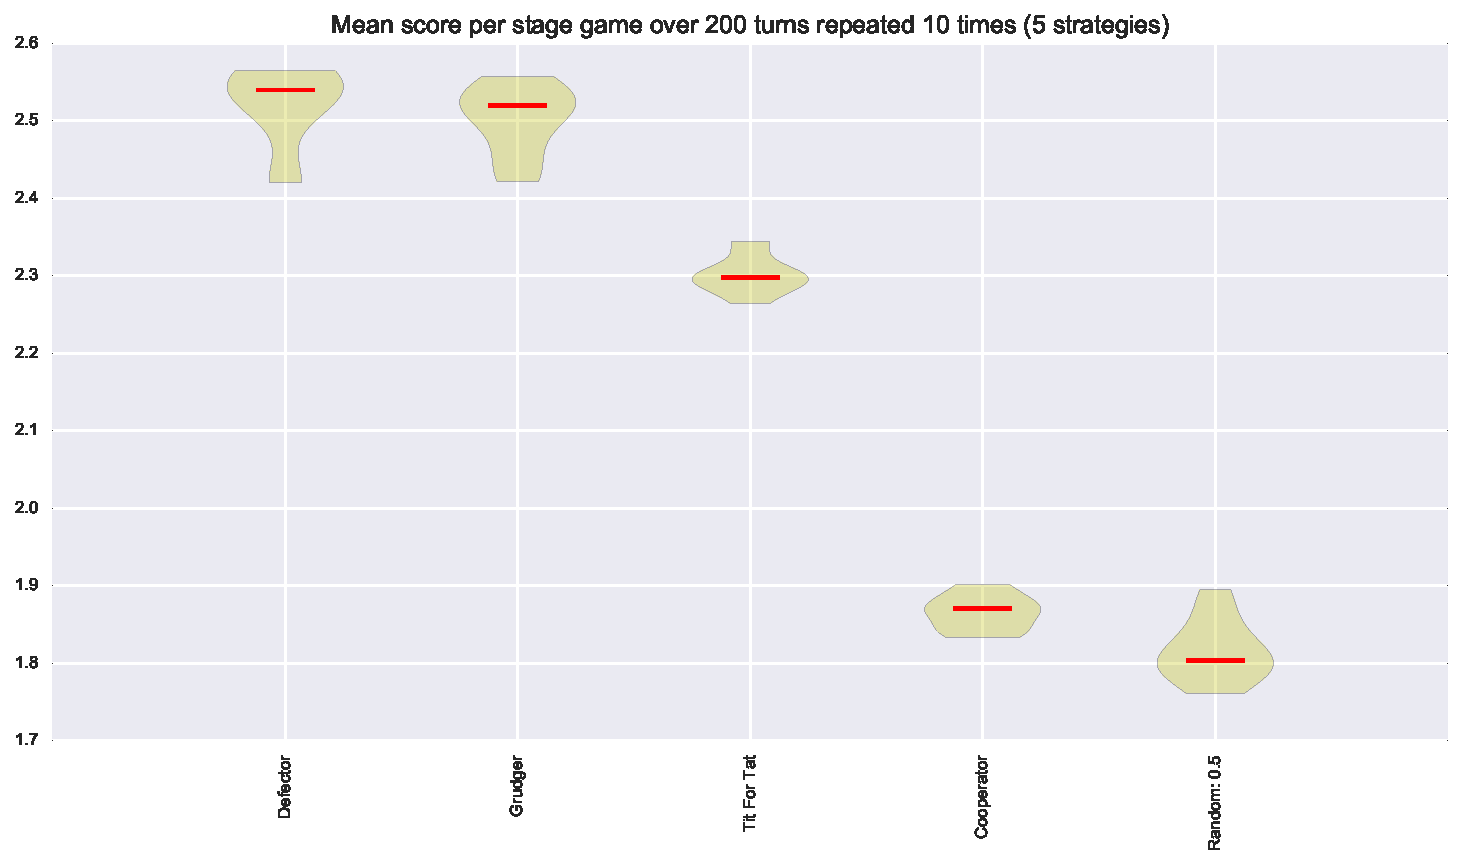
\includegraphics[width=.8\textwidth]{../img/demo_tournament.pdf}
    \caption{The results from a simple tournament.}
    \label{fig:demo_tournament}
\end{figure}

Figure \ref{fig:demo_tournament_commands} just shows the very basic utilisation
of the library and further details can be found at the online documentation:
\url{http://axelrod.readthedocs.org}. Some further implemented capabilities
include:

\begin{itemize}
    \item Noisy tournaments
    \item Ecological tournaments
    \item Full tournament history
    \item Creation of plots of distributions of scores and wins
\end{itemize}

As stated in Section~\ref{sec:introduction} one of the main goals of the library
is to allow for the easy contribution of strategies. To do this requires the
writing of a simple python class (which can inherit from other predefined
classes). Full contribution guidelines can be found in the documentation.
Figures~\ref{fig:grudger} and~\ref{fig:grudger_test} show the source code for
the Grudger strategy as well as its corresponding test.

\begin{figure}[!hbtp]
    \begin{minted}[breaklines, linenos, frame=lines]{python}
class Grudger(Player):
    """A player starts by cooperating however will defect if
       at any point the opponent has defected."""

    name = 'Grudger'
    classifier = {
        'memory_depth': float('inf'),  # Long memory
        'stochastic': False,
        'inspects_source': False,
        'manipulates_source': False,
        'manipulates_state': False
    }

    def strategy(self, opponent):
        """Begins by playing C, then plays D for the remaining
           rounds if the opponent ever plays D."""
        if opponent.defections:
            return D
        return C
    \end{minted}
    \caption{Source code for the Grudger strategy.}
    \label{fig:grudger}
\end{figure}


\begin{figure}[!hbtp]
    \begin{minted}[breaklines, linenos, frame=lines]{python}
class TestGrudger(TestPlayer):

    name = "Grudger"
    player = axelrod.Grudger
    expected_classifier = {
        'memory_depth': float('inf'),  # Long memory
        'stochastic': False,
        'inspects_source': False,
        'manipulates_source': False,
        'manipulates_state': False
    }

    def test_initial_strategy(self):
        """
        Starts by cooperating
        """
        self.first_play_test(C)

    def test_strategy(self):
        """
        If opponent defects at any point then the player will defect forever
        """
        self.responses_test([C, D, D, D], [C, C, C, C], [C])
        self.responses_test([C, C, D, D, D], [C, D, C, C, C], [D])
    \end{minted}
    \caption{Test code for the Grudger strategy.}
    \label{fig:grudger_test}
\end{figure}

You can see an overview of some of the source code in Figure~\ref{fig:overview}.

\begin{figure}[!hbtp]
    \centering
    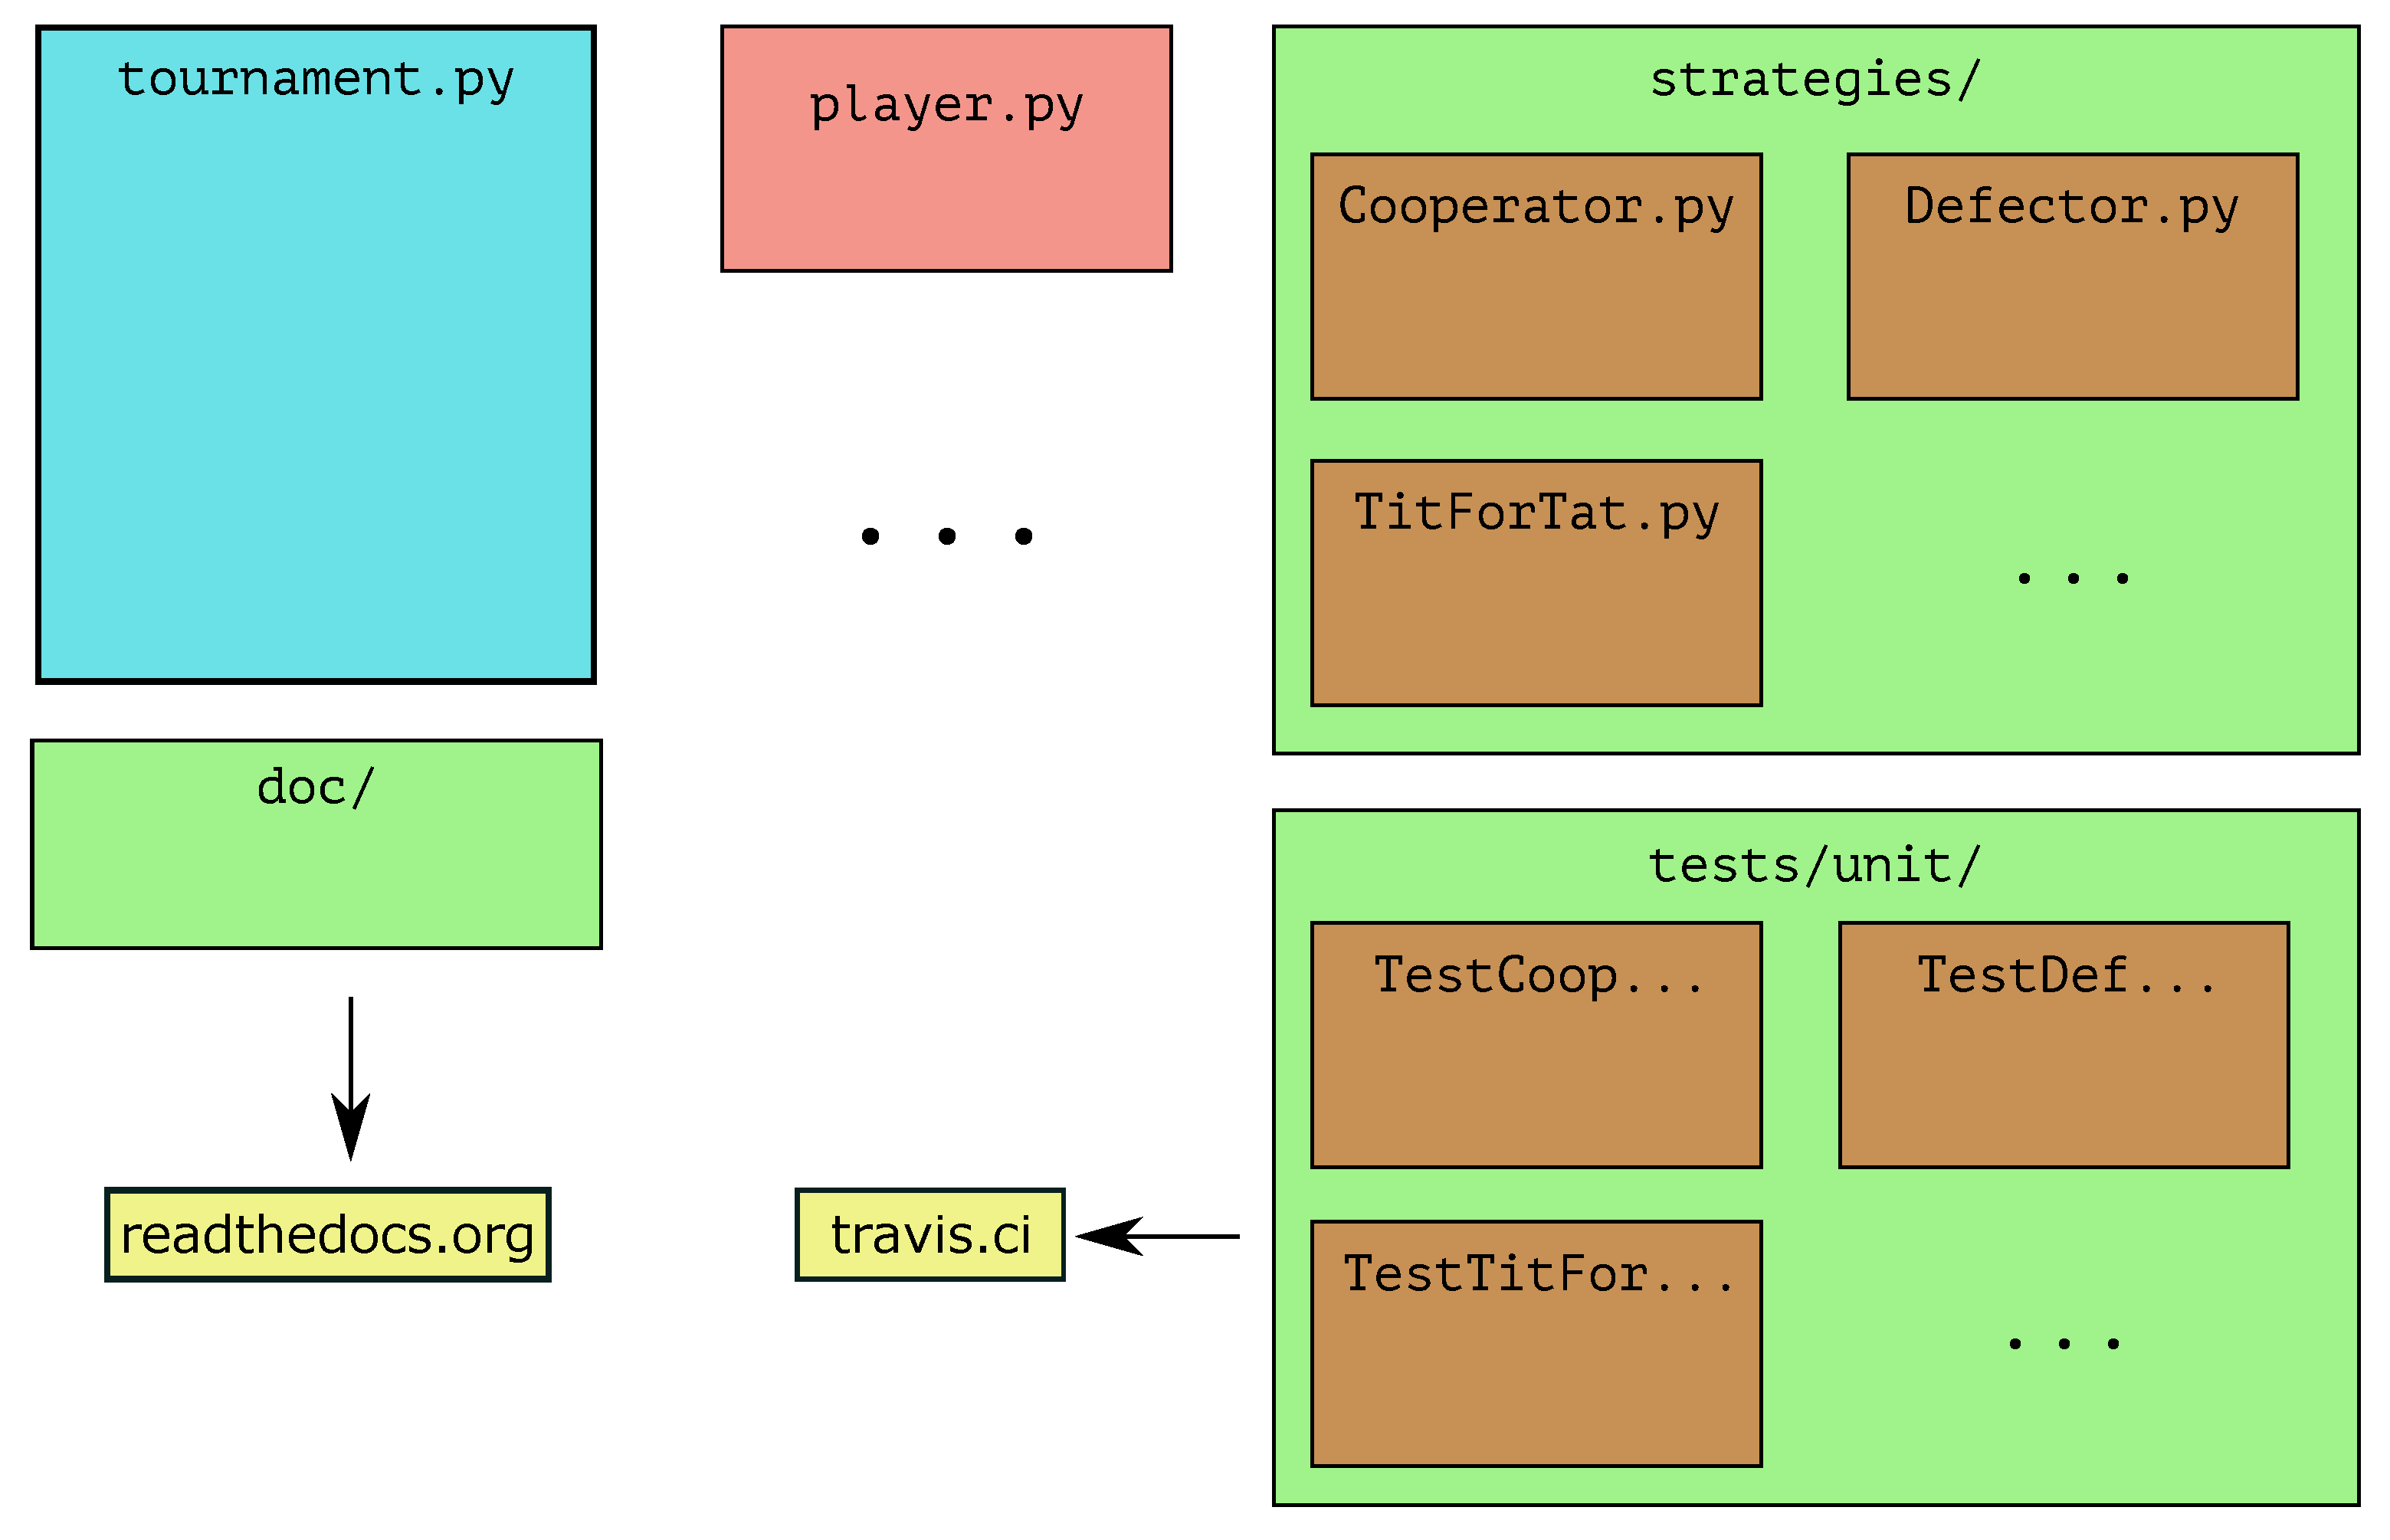
\includegraphics[width=.8\textwidth]{../img/outline_of_library.pdf}
    \caption{An overview of the source code.}
    \label{fig:overview}
\end{figure}

To date the library has had contributions from 19 contributors from a variety of
backgrounds. These contributions have both been in terms of strategies (one
strategy is the creation of an undergraduate mathematics student with little
prior knowledge of programming) as well as the architecture of the library
itself.

Before discussing the novel insights obtained from the study of this library in
Section~\ref{sec:new-strategies-and-implications} an overview of some
tournaments that have been reproduced will be given in
Section~\ref{sec:reproducing-previous-tournaments}.

\section{Reproducing previous tournaments}\label{sec:reproducing-previous-tournaments}

Stewart and Plotkin 2012 is fully reproducible; results are unstable (e.g.\
substituting \texttt{soft\_majo} for \texttt{hard\_majo} changes the results).

\section{New strategies, tournaments and implications}\label{sec:new-strategies-and-implications}

Ideas for this section:
* ZD strategies -- extortionate strategies win well but no ZDs score partiocualrly well,
even ZDGTFT2. With noise the ZD strategies don't win well either.
* TFT, T2FT, TF2T -- no so great but variants with e.g. deadlock breaking, such as OmegaTFT,
fare well
* It's posible to win many matchups as well score highly -- backstabber, doublecrosser,
foolmeonce. These strategies also score well in noisy tournaments
* It's possible to be generally cooperative and still exploit naive strategies effective,
such as LookerUp and MetaHunter
* Long memory strategies are generally better
* Meta strategies fare very well in general, also in noisy tournaments
* Variance of score distributions is surprisingly low

%Plot of memory_depth vs mean score, mean wins?

\section{Conclusion}\label{sec:conclusion}

\printbibliography
\end{document}
